% Options for packages loaded elsewhere
\PassOptionsToPackage{unicode}{hyperref}
\PassOptionsToPackage{hyphens}{url}
%
\documentclass[
]{article}
\title{NICE DSU Technical Support Document 18 - Appendix D}
\author{Aidan}
\date{07/01/2022}

\usepackage{amsmath,amssymb}
\usepackage{lmodern}
\usepackage{iftex}
\ifPDFTeX
  \usepackage[T1]{fontenc}
  \usepackage[utf8]{inputenc}
  \usepackage{textcomp} % provide euro and other symbols
\else % if luatex or xetex
  \usepackage{unicode-math}
  \defaultfontfeatures{Scale=MatchLowercase}
  \defaultfontfeatures[\rmfamily]{Ligatures=TeX,Scale=1}
\fi
% Use upquote if available, for straight quotes in verbatim environments
\IfFileExists{upquote.sty}{\usepackage{upquote}}{}
\IfFileExists{microtype.sty}{% use microtype if available
  \usepackage[]{microtype}
  \UseMicrotypeSet[protrusion]{basicmath} % disable protrusion for tt fonts
}{}
\makeatletter
\@ifundefined{KOMAClassName}{% if non-KOMA class
  \IfFileExists{parskip.sty}{%
    \usepackage{parskip}
  }{% else
    \setlength{\parindent}{0pt}
    \setlength{\parskip}{6pt plus 2pt minus 1pt}}
}{% if KOMA class
  \KOMAoptions{parskip=half}}
\makeatother
\usepackage{xcolor}
\IfFileExists{xurl.sty}{\usepackage{xurl}}{} % add URL line breaks if available
\IfFileExists{bookmark.sty}{\usepackage{bookmark}}{\usepackage{hyperref}}
\hypersetup{
  pdftitle={NICE DSU Technical Support Document 18 - Appendix D},
  pdfauthor={Aidan},
  hidelinks,
  pdfcreator={LaTeX via pandoc}}
\urlstyle{same} % disable monospaced font for URLs
\usepackage[margin=1in]{geometry}
\usepackage{color}
\usepackage{fancyvrb}
\newcommand{\VerbBar}{|}
\newcommand{\VERB}{\Verb[commandchars=\\\{\}]}
\DefineVerbatimEnvironment{Highlighting}{Verbatim}{commandchars=\\\{\}}
% Add ',fontsize=\small' for more characters per line
\usepackage{framed}
\definecolor{shadecolor}{RGB}{248,248,248}
\newenvironment{Shaded}{\begin{snugshade}}{\end{snugshade}}
\newcommand{\AlertTok}[1]{\textcolor[rgb]{0.94,0.16,0.16}{#1}}
\newcommand{\AnnotationTok}[1]{\textcolor[rgb]{0.56,0.35,0.01}{\textbf{\textit{#1}}}}
\newcommand{\AttributeTok}[1]{\textcolor[rgb]{0.77,0.63,0.00}{#1}}
\newcommand{\BaseNTok}[1]{\textcolor[rgb]{0.00,0.00,0.81}{#1}}
\newcommand{\BuiltInTok}[1]{#1}
\newcommand{\CharTok}[1]{\textcolor[rgb]{0.31,0.60,0.02}{#1}}
\newcommand{\CommentTok}[1]{\textcolor[rgb]{0.56,0.35,0.01}{\textit{#1}}}
\newcommand{\CommentVarTok}[1]{\textcolor[rgb]{0.56,0.35,0.01}{\textbf{\textit{#1}}}}
\newcommand{\ConstantTok}[1]{\textcolor[rgb]{0.00,0.00,0.00}{#1}}
\newcommand{\ControlFlowTok}[1]{\textcolor[rgb]{0.13,0.29,0.53}{\textbf{#1}}}
\newcommand{\DataTypeTok}[1]{\textcolor[rgb]{0.13,0.29,0.53}{#1}}
\newcommand{\DecValTok}[1]{\textcolor[rgb]{0.00,0.00,0.81}{#1}}
\newcommand{\DocumentationTok}[1]{\textcolor[rgb]{0.56,0.35,0.01}{\textbf{\textit{#1}}}}
\newcommand{\ErrorTok}[1]{\textcolor[rgb]{0.64,0.00,0.00}{\textbf{#1}}}
\newcommand{\ExtensionTok}[1]{#1}
\newcommand{\FloatTok}[1]{\textcolor[rgb]{0.00,0.00,0.81}{#1}}
\newcommand{\FunctionTok}[1]{\textcolor[rgb]{0.00,0.00,0.00}{#1}}
\newcommand{\ImportTok}[1]{#1}
\newcommand{\InformationTok}[1]{\textcolor[rgb]{0.56,0.35,0.01}{\textbf{\textit{#1}}}}
\newcommand{\KeywordTok}[1]{\textcolor[rgb]{0.13,0.29,0.53}{\textbf{#1}}}
\newcommand{\NormalTok}[1]{#1}
\newcommand{\OperatorTok}[1]{\textcolor[rgb]{0.81,0.36,0.00}{\textbf{#1}}}
\newcommand{\OtherTok}[1]{\textcolor[rgb]{0.56,0.35,0.01}{#1}}
\newcommand{\PreprocessorTok}[1]{\textcolor[rgb]{0.56,0.35,0.01}{\textit{#1}}}
\newcommand{\RegionMarkerTok}[1]{#1}
\newcommand{\SpecialCharTok}[1]{\textcolor[rgb]{0.00,0.00,0.00}{#1}}
\newcommand{\SpecialStringTok}[1]{\textcolor[rgb]{0.31,0.60,0.02}{#1}}
\newcommand{\StringTok}[1]{\textcolor[rgb]{0.31,0.60,0.02}{#1}}
\newcommand{\VariableTok}[1]{\textcolor[rgb]{0.00,0.00,0.00}{#1}}
\newcommand{\VerbatimStringTok}[1]{\textcolor[rgb]{0.31,0.60,0.02}{#1}}
\newcommand{\WarningTok}[1]{\textcolor[rgb]{0.56,0.35,0.01}{\textbf{\textit{#1}}}}
\usepackage{graphicx}
\makeatletter
\def\maxwidth{\ifdim\Gin@nat@width>\linewidth\linewidth\else\Gin@nat@width\fi}
\def\maxheight{\ifdim\Gin@nat@height>\textheight\textheight\else\Gin@nat@height\fi}
\makeatother
% Scale images if necessary, so that they will not overflow the page
% margins by default, and it is still possible to overwrite the defaults
% using explicit options in \includegraphics[width, height, ...]{}
\setkeys{Gin}{width=\maxwidth,height=\maxheight,keepaspectratio}
% Set default figure placement to htbp
\makeatletter
\def\fps@figure{htbp}
\makeatother
\setlength{\emergencystretch}{3em} % prevent overfull lines
\providecommand{\tightlist}{%
  \setlength{\itemsep}{0pt}\setlength{\parskip}{0pt}}
\setcounter{secnumdepth}{-\maxdimen} % remove section numbering
\ifLuaTeX
  \usepackage{selnolig}  % disable illegal ligatures
\fi

\begin{document}
\maketitle

\begin{Shaded}
\begin{Highlighting}[]
\FunctionTok{library}\NormalTok{(dplyr)}
\FunctionTok{library}\NormalTok{(tidyr)}
\FunctionTok{library}\NormalTok{(wakefield)}
\FunctionTok{library}\NormalTok{(ggplot2)}
\FunctionTok{library}\NormalTok{(sandwich)}

\FunctionTok{set.seed}\NormalTok{(}\DecValTok{1374988}\NormalTok{)}
\end{Highlighting}
\end{Shaded}

\hypertarget{background-and-resources}{%
\subsection{Background and resources}\label{background-and-resources}}

This report is a copy of the text and code shown in NICE's worked
example of MAIC and STC. The purpose of this notebook is to generate
data and reproduce NICE's analysis in R, to validate the results of this
Python implementation. Due to differences in system and package
versions, the data generated - and therefore the results - in this
analysis do not exactly match the original document (despite using the
same seed).

The text and code are lifted from the Appendix document below with
almost no modification. All credit for this R implementation goes to the
original authors.

\begin{itemize}
\tightlist
\item
  \href{http://nicedsu.org.uk/wp-content/uploads/2018/08/Population-adjustment-TSD-FINAL-ref-rerun.pdf}{NICE
  DSU Technical Support Document 18}
\item
  \href{http://nicedsu.org.uk/wp-content/uploads/2017/05/TSD18-Appendix-D-Worked-example-of-MAIC-and-STC.pdf}{Appendix
  D: Worked example of MAIC and STC}
\end{itemize}

\hypertarget{creating-simulated-datasets}{%
\subsection{Creating simulated
datasets}\label{creating-simulated-datasets}}

First, we create some simulated data. We use the package
\texttt{wakefield}, which provides an easy way to quickly create
realistic simulated datasets with pre-set variable types. We will
consider two variables, age and gender, with age being an effect
modifier and gender a purely prognostic variable.

Here, we set the parameters of the simulation scenario, defining study
characteristics (study sizes, age ranges, proportion of females) and the
parameters of the outcome model.

\begin{Shaded}
\begin{Highlighting}[]
\CommentTok{\# Study characteristics}
\NormalTok{N\_AB }\OtherTok{\textless{}{-}} \DecValTok{500}
\NormalTok{N\_AC }\OtherTok{\textless{}{-}} \DecValTok{300}
\NormalTok{agerange\_AB }\OtherTok{\textless{}{-}} \DecValTok{45}\SpecialCharTok{:}\DecValTok{75}
\NormalTok{agerange\_AC }\OtherTok{\textless{}{-}} \DecValTok{45}\SpecialCharTok{:}\DecValTok{55}
\NormalTok{femalepc\_AB }\OtherTok{\textless{}{-}} \FloatTok{0.64}
\NormalTok{femalepc\_AC }\OtherTok{\textless{}{-}} \FloatTok{0.8}

\CommentTok{\# Outcome model}
\NormalTok{b\_0 }\OtherTok{\textless{}{-}} \FloatTok{0.85}
\NormalTok{b\_gender }\OtherTok{\textless{}{-}} \FloatTok{0.12}
\NormalTok{b\_age }\OtherTok{\textless{}{-}} \FloatTok{0.05}
\NormalTok{b\_age\_trt }\OtherTok{\textless{}{-}} \SpecialCharTok{{-}}\FloatTok{0.08}
\NormalTok{b\_trt\_B }\OtherTok{\textless{}{-}} \SpecialCharTok{{-}}\FloatTok{2.1}
\NormalTok{b\_trt\_C }\OtherTok{\textless{}{-}} \SpecialCharTok{{-}}\FloatTok{2.5}
\end{Highlighting}
\end{Shaded}

For our example, we will generate binary outcomes. The true logistic
outcome model which we use to simulate the data will be:

\[logit(p_{it})=0.85+0.12\cdot\ male_{it}+0.05\cdot\ (age_{it}-40)+(\beta_{t}-0.08\cdot\ (age_{it}-40))\parallel(t\neq A)\]

where \(\beta_{B}=-2.1\) and \(\beta_{C}=-2.5\). The parameters of the
model are interpreted as log odds ratios, and \(p_{it}\) is the
probability of an event for individual \(i\) receiving treatment \(t\).

\hypertarget{ab-trial}{%
\subsubsection{AB trial}\label{ab-trial}}

The \(AB\) trial (\(N_{(AB)}=500\)) will have ages from 45 to 75 and
64\% females. The \texttt{wakefield} package provides a framework for
generating simulated datasets, including many convenience functions; we
make use of just a small number here, including age to uniformly
generate ages within an age range, gender to generate a factor variable
of genders with given probabilities, and id to create a unique ID for
each individual.

\begin{Shaded}
\begin{Highlighting}[]
\CommentTok{\# generate data for the AB trial}
\NormalTok{AB.IPD }\OtherTok{\textless{}{-}}
  \FunctionTok{rbind}\NormalTok{(}
    
    \CommentTok{\# Generate A arm}
    \FunctionTok{r\_data\_frame}\NormalTok{(}\AttributeTok{n =}\NormalTok{ N\_AB}\SpecialCharTok{/}\DecValTok{2}\NormalTok{, }\CommentTok{\# Number of individuals in arm A}
\NormalTok{                 id, }\CommentTok{\# Unique ID}
                 \AttributeTok{age =} \FunctionTok{age}\NormalTok{(}\AttributeTok{x =}\NormalTok{ agerange\_AB), }\CommentTok{\# Generate ages}
                 \AttributeTok{gender =} \FunctionTok{gender}\NormalTok{(}\AttributeTok{prob =} \FunctionTok{c}\NormalTok{(}\DecValTok{1} \SpecialCharTok{{-}}\NormalTok{ femalepc\_AB, femalepc\_AB)), }\CommentTok{\# Generate genders}
                 \AttributeTok{trt =} \StringTok{"A"} \CommentTok{\# Assign treatment A}
\NormalTok{    ),}
    
    \CommentTok{\# Generate B arm}
    \FunctionTok{r\_data\_frame}\NormalTok{(}\AttributeTok{n =}\NormalTok{ N\_AB}\SpecialCharTok{/}\DecValTok{2}\NormalTok{, }\CommentTok{\# Number of individuals in arm B}
\NormalTok{                 id, }\CommentTok{\# Unique ID}
                 \AttributeTok{age =} \FunctionTok{age}\NormalTok{(}\AttributeTok{x =}\NormalTok{ agerange\_AB), }\CommentTok{\# Generate ages}
                 \AttributeTok{gender =} \FunctionTok{gender}\NormalTok{(}\AttributeTok{prob =} \FunctionTok{c}\NormalTok{(}\DecValTok{1} \SpecialCharTok{{-}}\NormalTok{ femalepc\_AB, femalepc\_AB)), }\CommentTok{\# Generate genders}
                 \AttributeTok{trt =} \StringTok{"B"} \CommentTok{\# Assign treatment B}
\NormalTok{    )}
\NormalTok{  ) }\SpecialCharTok{\%\textgreater{}\%}
  
  \CommentTok{\# Generate outcomes using logistic model}
  \FunctionTok{mutate}\NormalTok{(}
    \AttributeTok{yprob =} \DecValTok{1} \SpecialCharTok{/}\NormalTok{ (}\DecValTok{1} \SpecialCharTok{+} \FunctionTok{exp}\NormalTok{(}\SpecialCharTok{{-}}\NormalTok{(}
\NormalTok{      b\_0 }\SpecialCharTok{+}\NormalTok{ b\_gender }\SpecialCharTok{*}\NormalTok{ (gender }\SpecialCharTok{==} \StringTok{"Male"}\NormalTok{) }\SpecialCharTok{+}\NormalTok{ b\_age }\SpecialCharTok{*}\NormalTok{ (age }\SpecialCharTok{{-}} \DecValTok{40}\NormalTok{) }\SpecialCharTok{+}
        \FunctionTok{if\_else}\NormalTok{(trt }\SpecialCharTok{==} \StringTok{"B"}\NormalTok{, b\_trt\_B }\SpecialCharTok{+}\NormalTok{ b\_age\_trt }\SpecialCharTok{*}\NormalTok{ (age }\SpecialCharTok{{-}} \DecValTok{40}\NormalTok{), }\DecValTok{0}\NormalTok{)}
\NormalTok{    ))),}
    \AttributeTok{y =} \FunctionTok{rbinom}\NormalTok{(N\_AB, }\DecValTok{1}\NormalTok{, yprob)}
\NormalTok{  ) }\SpecialCharTok{\%\textgreater{}\%}
  \FunctionTok{select}\NormalTok{(}\SpecialCharTok{{-}}\NormalTok{yprob) }\CommentTok{\# Drop the yprob column}

\FunctionTok{write.csv}\NormalTok{(AB.IPD, }\AttributeTok{file=}\StringTok{"..}\SpecialCharTok{\textbackslash{}\textbackslash{}}\StringTok{data}\SpecialCharTok{\textbackslash{}\textbackslash{}}\StringTok{AB\_IPD.csv"}\NormalTok{, }\AttributeTok{row.names=}\ConstantTok{FALSE}\NormalTok{)}
\end{Highlighting}
\end{Shaded}

Tabulate the AB trial, to check that our ``randomisation'' has worked,
and examine the generated outcomes.

\begin{Shaded}
\begin{Highlighting}[]
\NormalTok{AB.IPD }\SpecialCharTok{\%\textgreater{}\%} \FunctionTok{group\_by}\NormalTok{(trt) }\SpecialCharTok{\%\textgreater{}\%}
  \FunctionTok{summarise}\NormalTok{(}\FunctionTok{n}\NormalTok{(), }\FunctionTok{mean}\NormalTok{(age), }\FunctionTok{sd}\NormalTok{(age), }\StringTok{\textasciigrave{}}\AttributeTok{n(male)}\StringTok{\textasciigrave{}}\OtherTok{=}\FunctionTok{sum}\NormalTok{(gender}\SpecialCharTok{==}\StringTok{"Male"}\NormalTok{),}
            \StringTok{\textasciigrave{}}\AttributeTok{\%(male)}\StringTok{\textasciigrave{}}\OtherTok{=}\FunctionTok{mean}\NormalTok{(gender}\SpecialCharTok{==}\StringTok{"Male"}\NormalTok{), }\FunctionTok{sum}\NormalTok{(y), }\FunctionTok{mean}\NormalTok{(y))}
\end{Highlighting}
\end{Shaded}

\begin{verbatim}
## # A tibble: 2 x 8
##   trt   `n()` `mean(age)` `sd(age)` `n(male)` `%(male)` `sum(y)` `mean(y)`
##   <chr> <int>       <dbl>     <dbl>     <int>     <dbl>    <int>     <dbl>
## 1 A       250        60.5      9.01        99     0.396      221     0.884
## 2 B       250        59.9      9.06        90     0.36        41     0.164
\end{verbatim}

\hypertarget{ac-trial}{%
\subsubsection{AC trial}\label{ac-trial}}

The \(AC\) trial (\(N_{(AC)}=300\)) will have ages from 45 to 55 and
80\% females.

\begin{Shaded}
\begin{Highlighting}[]
\CommentTok{\# generate data for the AC trial}
\NormalTok{AC.IPD }\OtherTok{\textless{}{-}}
  \FunctionTok{rbind}\NormalTok{(}
    
    \CommentTok{\# Generate A arm}
    \FunctionTok{r\_data\_frame}\NormalTok{(}\AttributeTok{n =}\NormalTok{ N\_AC}\SpecialCharTok{/}\DecValTok{2}\NormalTok{, }\CommentTok{\# Number of individuals in arm A}
\NormalTok{                 id, }\CommentTok{\# Unique ID}
                 \AttributeTok{age =} \FunctionTok{age}\NormalTok{(}\AttributeTok{x =}\NormalTok{ agerange\_AC), }\CommentTok{\# Generate ages}
                 \AttributeTok{gender =} \FunctionTok{gender}\NormalTok{(}\AttributeTok{prob =} \FunctionTok{c}\NormalTok{(}\DecValTok{1} \SpecialCharTok{{-}}\NormalTok{ femalepc\_AC, femalepc\_AC)), }\CommentTok{\# Generate genders}
                 \AttributeTok{trt =} \StringTok{"A"} \CommentTok{\# Assign treatment A}
\NormalTok{    ),}
    
    \CommentTok{\# Generate C arm}
    \FunctionTok{r\_data\_frame}\NormalTok{(}\AttributeTok{n =}\NormalTok{ N\_AC}\SpecialCharTok{/}\DecValTok{2}\NormalTok{, }\CommentTok{\# Number of individuals in arm C}
\NormalTok{                 id, }\CommentTok{\# Unique ID}
                 \AttributeTok{age =} \FunctionTok{age}\NormalTok{(}\AttributeTok{x =}\NormalTok{ agerange\_AC), }\CommentTok{\# Generate ages}
                 \AttributeTok{gender =} \FunctionTok{gender}\NormalTok{(}\AttributeTok{prob =} \FunctionTok{c}\NormalTok{(}\DecValTok{1} \SpecialCharTok{{-}}\NormalTok{ femalepc\_AC, femalepc\_AC)), }\CommentTok{\# Generate genders}
                 \AttributeTok{trt =} \StringTok{"C"} \CommentTok{\# Assign treatment C}
\NormalTok{    )}
\NormalTok{  ) }\SpecialCharTok{\%\textgreater{}\%}
  
  \CommentTok{\# Generate outcomes using logistic model}
  \FunctionTok{mutate}\NormalTok{(}
    \AttributeTok{yprob =} \DecValTok{1} \SpecialCharTok{/}\NormalTok{ (}\DecValTok{1} \SpecialCharTok{+} \FunctionTok{exp}\NormalTok{(}\SpecialCharTok{{-}}\NormalTok{(}
\NormalTok{      b\_0 }\SpecialCharTok{+}\NormalTok{ b\_gender }\SpecialCharTok{*}\NormalTok{ (gender }\SpecialCharTok{==} \StringTok{"Male"}\NormalTok{) }\SpecialCharTok{+}\NormalTok{ b\_age }\SpecialCharTok{*}\NormalTok{ (age }\SpecialCharTok{{-}} \DecValTok{40}\NormalTok{) }\SpecialCharTok{+}
        \FunctionTok{if\_else}\NormalTok{(trt }\SpecialCharTok{==} \StringTok{"C"}\NormalTok{, b\_trt\_C }\SpecialCharTok{+}\NormalTok{ b\_age\_trt }\SpecialCharTok{*}\NormalTok{ (age }\SpecialCharTok{{-}} \DecValTok{40}\NormalTok{), }\DecValTok{0}\NormalTok{)}
\NormalTok{    ))),}
    \AttributeTok{y =} \FunctionTok{rbinom}\NormalTok{(N\_AC, }\DecValTok{1}\NormalTok{, yprob)}
\NormalTok{  ) }\SpecialCharTok{\%\textgreater{}\%}
  \FunctionTok{select}\NormalTok{(}\SpecialCharTok{{-}}\NormalTok{yprob) }\CommentTok{\# Drop the yprob column}
\end{Highlighting}
\end{Shaded}

Tabulate the AC trial, to check that our ``randomisation'' has worked,
and examine the generated outcomes.

\begin{Shaded}
\begin{Highlighting}[]
\NormalTok{AC.IPD }\SpecialCharTok{\%\textgreater{}\%} \FunctionTok{group\_by}\NormalTok{(trt) }\SpecialCharTok{\%\textgreater{}\%}
  \FunctionTok{summarise}\NormalTok{(}\FunctionTok{n}\NormalTok{(), }\FunctionTok{mean}\NormalTok{(age), }\FunctionTok{sd}\NormalTok{(age), }\StringTok{\textasciigrave{}}\AttributeTok{n(male)}\StringTok{\textasciigrave{}}\OtherTok{=}\FunctionTok{sum}\NormalTok{(gender}\SpecialCharTok{==}\StringTok{"Male"}\NormalTok{),}
            \StringTok{\textasciigrave{}}\AttributeTok{\%(male)}\StringTok{\textasciigrave{}}\OtherTok{=}\FunctionTok{mean}\NormalTok{(gender}\SpecialCharTok{==}\StringTok{"Male"}\NormalTok{), }\FunctionTok{sum}\NormalTok{(y), }\FunctionTok{mean}\NormalTok{(y))}
\end{Highlighting}
\end{Shaded}

\begin{verbatim}
## # A tibble: 2 x 8
##   trt   `n()` `mean(age)` `sd(age)` `n(male)` `%(male)` `sum(y)` `mean(y)`
##   <chr> <int>       <dbl>     <dbl>     <int>     <dbl>    <int>     <dbl>
## 1 A       150        50.4      3.06        32     0.213      125     0.833
## 2 C       150        50.2      3.20        36     0.24        21     0.14
\end{verbatim}

For analysis we will have access only to the aggregate data, as if from
a published study. Here, we aggregate the IPD to obtain summaries, which
will be used for the MAIC and STC analyses.

\begin{Shaded}
\begin{Highlighting}[]
\CommentTok{\# aggregate AC trial data}
\NormalTok{AC.AgD }\OtherTok{\textless{}{-}}
  \FunctionTok{cbind}\NormalTok{(}
    \CommentTok{\# Trial level stats: mean and sd of age, number and proportion of males}
    \FunctionTok{summarise}\NormalTok{(AC.IPD, }\AttributeTok{age.mean =} \FunctionTok{mean}\NormalTok{(age), }\AttributeTok{age.sd =} \FunctionTok{sd}\NormalTok{(age),}
              \AttributeTok{N.male =} \FunctionTok{sum}\NormalTok{(gender}\SpecialCharTok{==}\StringTok{"Male"}\NormalTok{), }\AttributeTok{prop.male =} \FunctionTok{mean}\NormalTok{(gender}\SpecialCharTok{==}\StringTok{"Male"}\NormalTok{)),}
    \CommentTok{\# Summary outcomes for A arm}
    \FunctionTok{filter}\NormalTok{(AC.IPD, trt }\SpecialCharTok{==} \StringTok{"A"}\NormalTok{) }\SpecialCharTok{\%\textgreater{}\%}
      \FunctionTok{summarise}\NormalTok{(}\AttributeTok{y.A.sum =} \FunctionTok{sum}\NormalTok{(y), }\AttributeTok{y.A.bar =} \FunctionTok{mean}\NormalTok{(y), }\AttributeTok{N.A =} \FunctionTok{n}\NormalTok{()),}
    \CommentTok{\# Summary outcomes for C arm}
    \FunctionTok{filter}\NormalTok{(AC.IPD, trt }\SpecialCharTok{==} \StringTok{"C"}\NormalTok{) }\SpecialCharTok{\%\textgreater{}\%}
      \FunctionTok{summarise}\NormalTok{(}\AttributeTok{y.C.sum =} \FunctionTok{sum}\NormalTok{(y), }\AttributeTok{y.C.bar =} \FunctionTok{mean}\NormalTok{(y), }\AttributeTok{N.C =} \FunctionTok{n}\NormalTok{())}
\NormalTok{  )}

\FunctionTok{write.csv}\NormalTok{(AC.AgD, }\AttributeTok{file=}\StringTok{"..}\SpecialCharTok{\textbackslash{}\textbackslash{}}\StringTok{data}\SpecialCharTok{\textbackslash{}\textbackslash{}}\StringTok{AC\_AgD.csv"}\NormalTok{, }\AttributeTok{row.names=}\ConstantTok{FALSE}\NormalTok{)}
\NormalTok{AC.AgD}
\end{Highlighting}
\end{Shaded}

\begin{verbatim}
##   age.mean   age.sd N.male prop.male y.A.sum   y.A.bar N.A y.C.sum y.C.bar N.C
## 1 50.27333 3.124821     68 0.2266667     125 0.8333333 150      21    0.14 150
\end{verbatim}

\hypertarget{maic}{%
\subsection{MAIC}\label{maic}}

We are now ready to proceed with our analyses. First, we will estimate
the population-adjusted indirect comparison using MAIC. This involves
estimating a logistic propensity score model, which includes all effect
modifiers but no prognostic variables. This is equivalent to the
following model on the log of the individual weights:

\[log(w_{it}=\alpha_{0}+\alpha_{1}^TX_{it}^{EM}\]

The weights are estimated using the method of moments to match the
effect modifier distributions between the \(AB\) and \(AC\) trials. This
is equivalent to minimising

\[\sum_{i,t}exp(\alpha_{1}^TX_{it}^{EM})\]

when \(X_{(AC)}^{EM}=0\)

In order to do this, we define the objective function to minimise (as
above), and the gradient function (its derivative) which will be used by
the minimisation algorithm.

\begin{Shaded}
\begin{Highlighting}[]
\NormalTok{objfn }\OtherTok{\textless{}{-}} \ControlFlowTok{function}\NormalTok{(a1, X)\{}
  \FunctionTok{sum}\NormalTok{(}\FunctionTok{exp}\NormalTok{(X }\SpecialCharTok{\%*\%}\NormalTok{ a1))}
\NormalTok{\}}

\NormalTok{gradfn }\OtherTok{\textless{}{-}} \ControlFlowTok{function}\NormalTok{(a1, X)\{}
  \FunctionTok{colSums}\NormalTok{(}\FunctionTok{sweep}\NormalTok{(X, }\DecValTok{1}\NormalTok{, }\FunctionTok{exp}\NormalTok{(X }\SpecialCharTok{\%*\%}\NormalTok{ a1), }\StringTok{"*"}\NormalTok{))}
\NormalTok{\}}
\end{Highlighting}
\end{Shaded}

To satisfy \(\bar{X}_{AC}^{EM}=0\), we create centred versions of the
effect modifiers by subtracting \(\bar{X}_{AC}^{EM}\) from \(X^{EM}\) in
both trials. Here only age is an effect modifier, and we can balance
this in both mean and standard deviation as we have observed
\texttt{age.mean} and \texttt{age.sd} in the \(AC\) trial. We therefore
include centred versions of \texttt{age} and \texttt{ageˆ2} for each
individual in the \(AB\) trial in the weighting model. Centring the mean
is simple, but centring higher moments requires some attention: due to
aggregation, we cannot simply centre \texttt{ageˆ2} from the \(AB\)
trial with \texttt{age.sd} from the \(AC\) trial. We use the variance
formula \(var(X)=\mathbb{E}(X^2)-\mathbb{E}(X)^2\), and centre
\texttt{ageˆ2} in the \(AB\) trial with \texttt{age.meanˆ2\ +\ age.sdˆ2}
in the \(AC\) trial. Here we make use of the \texttt{sweep} function to
simultaneously centre the two row vectors \texttt{age} and
\texttt{ageˆ2} by subtracting \texttt{age.mean} and
\texttt{age.meanˆ2\ +\ age.sdˆ2} respectively:

\begin{Shaded}
\begin{Highlighting}[]
\NormalTok{X.EM}\FloatTok{.0} \OtherTok{\textless{}{-}} \FunctionTok{sweep}\NormalTok{(}\FunctionTok{with}\NormalTok{(AB.IPD, }\FunctionTok{cbind}\NormalTok{(age, age}\SpecialCharTok{\^{}}\DecValTok{2}\NormalTok{)), }\DecValTok{2}\NormalTok{,}
                \FunctionTok{with}\NormalTok{(AC.AgD, }\FunctionTok{c}\NormalTok{(age.mean, age.mean}\SpecialCharTok{\^{}}\DecValTok{2} \SpecialCharTok{+}\NormalTok{ age.sd}\SpecialCharTok{\^{}}\DecValTok{2}\NormalTok{)), }\StringTok{\textquotesingle{}{-}\textquotesingle{}}\NormalTok{)}
\end{Highlighting}
\end{Shaded}

To estimate \(\alpha_{1}\), we use the function \texttt{optim} to
minimise the function \texttt{objfn}. The method we tell optim to use is
BFGS (after Broyden, Fletcher, Goldfarb and Shanno), which makes use of
the gradient function \texttt{gradfn} we specified to aid minimisation.
We have to specify an initial value in the par argument (we choose
\texttt{c(0,0)} here), and \(X=X.EM.0\) is passed to \texttt{objfn} and
\texttt{gradfn} as an additional argument.

\begin{Shaded}
\begin{Highlighting}[]
\FunctionTok{print}\NormalTok{(opt1 }\OtherTok{\textless{}{-}} \FunctionTok{optim}\NormalTok{(}\AttributeTok{par =} \FunctionTok{c}\NormalTok{(}\DecValTok{0}\NormalTok{,}\DecValTok{0}\NormalTok{), }\AttributeTok{fn =}\NormalTok{ objfn, }\AttributeTok{gr =}\NormalTok{ gradfn, }\AttributeTok{X =}\NormalTok{ X.EM}\FloatTok{.0}\NormalTok{, }\AttributeTok{method =} \StringTok{"BFGS"}\NormalTok{))}
\end{Highlighting}
\end{Shaded}

\begin{verbatim}
## $par
## [1]  3.68798519 -0.03696784
## 
## $value
## [1] 196.4207
## 
## $counts
## function gradient 
##       68       14 
## 
## $convergence
## [1] 0
## 
## $message
## NULL
\end{verbatim}

\begin{Shaded}
\begin{Highlighting}[]
\NormalTok{a1 }\OtherTok{\textless{}{-}}\NormalTok{ opt1}\SpecialCharTok{$}\NormalTok{par}
\end{Highlighting}
\end{Shaded}

The output generated simply states that convergence has occurred
successfully (\texttt{\$convergence\ =\ 0}). The estimate
\(\hat{\alpha}_{1}\) is found in \texttt{\$par}. (The other outputs are
\texttt{\$value}, the value of \texttt{objfn} at the minimum,
\texttt{\$counts}, the number of evaluations of \texttt{objfn} and
\texttt{gradfn} before convergence, and \texttt{\$message}, for any
additional information from the minimisation algorithm.)

The estimated weights for each individual are then found by
\(\hat{w_{it}}=exp(X_{it}^{EM}\hat{\alpha_1})\). We do not need to
estimate \(\alpha_{0}\), as this constant cancels out.

\begin{Shaded}
\begin{Highlighting}[]
\NormalTok{wt }\OtherTok{\textless{}{-}} \FunctionTok{exp}\NormalTok{(X.EM}\FloatTok{.0} \SpecialCharTok{\%*\%}\NormalTok{ a1)}
\end{Highlighting}
\end{Shaded}

It is easier to examine the distribution of the weights by scaling them,
so that the rescaled weights are relative to the original unit weights
of each individual; in other words, a rescaled weight \textgreater{} 1
means that an individual carries more weight in the reweighted
population than in the \(AB\) population, and a rescaled weight
\textless{} 1 means that an individual carries less weight. The rescaled
weight is calculated as

\[\tilde{w_{it}}=\frac{\hat{w_{it}}}{\sum_{i,t}\hat{w_{it}}}\cdot N_{(AB)}\]

\begin{Shaded}
\begin{Highlighting}[]
\NormalTok{wt.rs }\OtherTok{\textless{}{-}}\NormalTok{ (wt }\SpecialCharTok{/} \FunctionTok{sum}\NormalTok{(wt)) }\SpecialCharTok{*}\NormalTok{ N\_AB  }\CommentTok{\# rescaled weights}

\FunctionTok{summary}\NormalTok{(wt.rs)}
\end{Highlighting}
\end{Shaded}

\begin{verbatim}
##        V1         
##  Min.   :0.00000  
##  1st Qu.:0.00002  
##  Median :0.03803  
##  Mean   :1.00000  
##  3rd Qu.:2.10475  
##  Max.   :3.67109
\end{verbatim}

\begin{Shaded}
\begin{Highlighting}[]
\FunctionTok{qplot}\NormalTok{(wt.rs, }\AttributeTok{geom=}\StringTok{"histogram"}\NormalTok{,}
      \AttributeTok{xlab =} \StringTok{"Rescaled weight (multiple of original unit weight)"}\NormalTok{,}
      \AttributeTok{binwidth=}\FloatTok{0.25}\NormalTok{)}
\end{Highlighting}
\end{Shaded}

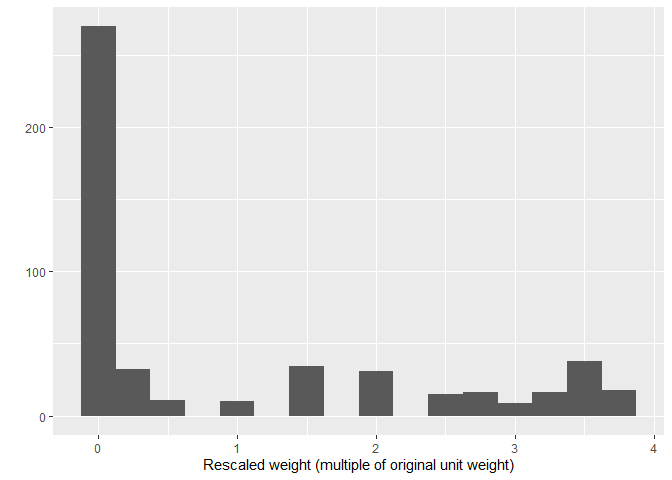
\includegraphics{NICE_DSU_Technical_Support_Document-Appendix_D_files/figure-latex/plot_weights-1.pdf}

The mean of the rescaled weights is not informative, as it is guaranteed
to be 1:

\[\frac{1}{N_{(AB)}}\sum_{i,t}\tilde{w_{it}}=\frac{1}{N_{(AB)}}\sum_{i,t}\frac{\hat{w_{it}}}{\sum_{i,t}\hat{w_{it}}}\cdot N_{(AB)}=1\]

Here, the rescaled weights range from 0 to 3.44, and the median is
heavily skewed towards zero (0.07). A histogram of the weights is also
very helpful to present, and clearly shows that a large number of
individuals have been given zero (or close to zero) weight. This is not
surprising, as the age range in the \(AB\) trial (45 to 75) is much
wider than that in the \(AC\) trial (45 to 55). There are therefore a
large number of individuals from the \(AB\) trial who have been
excluded. More positively, there are no very large weights, as the
distribution of effect modifiers in the \(AC\) population is entirely
contained within that of the \(AB\) population (there are no ages in the
\(AC\) population outside of those observed in the \(AB\) population).

The approximate effective sample size is calculated as

\[\frac{\sum_{i,t}(\hat{w_{it}})^2}{\sum_{i,t}\hat{w_{i,t}^2}}\]

\begin{Shaded}
\begin{Highlighting}[]
\FunctionTok{sum}\NormalTok{(wt)}\SpecialCharTok{\^{}}\DecValTok{2}\SpecialCharTok{/}\FunctionTok{sum}\NormalTok{(wt}\SpecialCharTok{\^{}}\DecValTok{2}\NormalTok{)}
\end{Highlighting}
\end{Shaded}

\begin{verbatim}
## [1] 178.5609
\end{verbatim}

This is quite a reduction from the original 500, but is still reasonably
large. (The actual ESS is likely to be larger than this, as the weights
are not fixed and known -- see section 2.2.1.)

Note that age is balanced (in terms of mean and SD) with the \(AC\)
population after weighting.

\begin{Shaded}
\begin{Highlighting}[]
\NormalTok{AB.IPD }\SpecialCharTok{\%\textgreater{}\%}
  \FunctionTok{mutate}\NormalTok{(wt) }\SpecialCharTok{\%\textgreater{}\%}
  \FunctionTok{summarise}\NormalTok{(}\AttributeTok{age.mean =} \FunctionTok{weighted.mean}\NormalTok{(age, wt),}
            \AttributeTok{age.sd =} \FunctionTok{sqrt}\NormalTok{(}\FunctionTok{sum}\NormalTok{(wt }\SpecialCharTok{/} \FunctionTok{sum}\NormalTok{(wt) }\SpecialCharTok{*}\NormalTok{ (age }\SpecialCharTok{{-}}\NormalTok{ age.mean)}\SpecialCharTok{\^{}}\DecValTok{2}\NormalTok{))}
\NormalTok{)}
\end{Highlighting}
\end{Shaded}

\begin{verbatim}
## # A tibble: 1 x 2
##   age.mean age.sd
##      <dbl>  <dbl>
## 1     50.3   3.12
\end{verbatim}

\begin{Shaded}
\begin{Highlighting}[]
\NormalTok{AC.AgD[, }\FunctionTok{c}\NormalTok{(}\StringTok{"age.mean"}\NormalTok{, }\StringTok{"age.sd"}\NormalTok{)]}
\end{Highlighting}
\end{Shaded}

\begin{verbatim}
##   age.mean   age.sd
## 1 50.27333 3.124821
\end{verbatim}

The estimated relative effect \(\hat{d}_{AB(AC)}\) of \(B\) vs.~\(A\) in
the \(AC\) population is found by taking weighted means of the outcomes
in the \(AB\) trial. However, in practice it is easier to generate these
estimates using a simple linear model: this is exactly equivalent to
taking the weighted means, but allows us to use the \texttt{sandwich}
package to calculate standard errors correctly using a sandwich
estimator. (Note that it is possible to generate estimates of absolute
outcomes on each treatment using the weighted means or the linear model,
but these will be biased unless all prognostic variables and effect
modifiers in imbalance between the populations are accounted for.
Unbiased prediction of absolute outcomes relies on the much stronger
assumption of conditional constancy of absolute effects.)

\begin{Shaded}
\begin{Highlighting}[]
\CommentTok{\# Binomial GLM}
\NormalTok{fit1 }\OtherTok{\textless{}{-}}
\NormalTok{AB.IPD }\SpecialCharTok{\%\textgreater{}\%} \FunctionTok{mutate}\NormalTok{(}\AttributeTok{y0 =} \DecValTok{1} \SpecialCharTok{{-}}\NormalTok{ y, }\AttributeTok{wt =}\NormalTok{ wt) }\SpecialCharTok{\%\textgreater{}\%}
\FunctionTok{glm}\NormalTok{(}\FunctionTok{cbind}\NormalTok{(y,y0) }\SpecialCharTok{\textasciitilde{}}\NormalTok{ trt, }\AttributeTok{data =}\NormalTok{ ., }\AttributeTok{family =}\NormalTok{ binomial, }\AttributeTok{weights =}\NormalTok{ wt)}
\CommentTok{\# Sandwich estimator of variance matrix}
\NormalTok{V.sw }\OtherTok{\textless{}{-}} \FunctionTok{vcovHC}\NormalTok{(fit1)}
\CommentTok{\# The log OR of B vs. A is just the trtB parameter estimate,}
\CommentTok{\# since effect modifiers were centred}
\FunctionTok{print}\NormalTok{(d.AB.MAIC }\OtherTok{\textless{}{-}} \FunctionTok{coef}\NormalTok{(fit1)[}\StringTok{"trtB"}\NormalTok{])}
\end{Highlighting}
\end{Shaded}

\begin{verbatim}
##      trtB 
## -3.385924
\end{verbatim}

\begin{Shaded}
\begin{Highlighting}[]
\FunctionTok{print}\NormalTok{(var.d.AB.MAIC }\OtherTok{\textless{}{-}}\NormalTok{ V.sw[}\StringTok{"trtB"}\NormalTok{,}\StringTok{"trtB"}\NormalTok{])}
\end{Highlighting}
\end{Shaded}

\begin{verbatim}
## [1] 0.170214
\end{verbatim}

Finally, we construct the indirect comparison estimate
\(\hat{d}_{BC(AC)}\) on the log OR scale, using the fact that
\(d_{BC(AC)}=d_{AC(AC)}-d_{AB(AC)}\).

\begin{Shaded}
\begin{Highlighting}[]
\CommentTok{\# Estimated log OR of C vs. A from the AC trial}
\NormalTok{d.AC }\OtherTok{\textless{}{-}} \FunctionTok{with}\NormalTok{(AC.AgD, }\FunctionTok{log}\NormalTok{(y.C.sum }\SpecialCharTok{*}\NormalTok{ (N.A }\SpecialCharTok{{-}}\NormalTok{ y.A.sum) }\SpecialCharTok{/}\NormalTok{ (y.A.sum }\SpecialCharTok{*}\NormalTok{ (N.C }\SpecialCharTok{{-}}\NormalTok{ y.C.sum))))}
\NormalTok{var.d.AC }\OtherTok{\textless{}{-}} \FunctionTok{with}\NormalTok{(AC.AgD, }\DecValTok{1}\SpecialCharTok{/}\NormalTok{y.A.sum }\SpecialCharTok{+} \DecValTok{1}\SpecialCharTok{/}\NormalTok{(N.A }\SpecialCharTok{{-}}\NormalTok{ y.A.sum) }\SpecialCharTok{+} \DecValTok{1}\SpecialCharTok{/}\NormalTok{y.C.sum }\SpecialCharTok{+} \DecValTok{1}\SpecialCharTok{/}\NormalTok{(N.C }\SpecialCharTok{{-}}\NormalTok{ y.C.sum))}

\CommentTok{\# Indirect comparison}
\FunctionTok{print}\NormalTok{(d.BC.MAIC }\OtherTok{\textless{}{-}}\NormalTok{ d.AC }\SpecialCharTok{{-}}\NormalTok{ d.AB.MAIC)}
\end{Highlighting}
\end{Shaded}

\begin{verbatim}
##        trtB 
## -0.03880351
\end{verbatim}

\begin{Shaded}
\begin{Highlighting}[]
\FunctionTok{print}\NormalTok{(var.d.BC.MAIC }\OtherTok{\textless{}{-}}\NormalTok{ var.d.AC }\SpecialCharTok{+}\NormalTok{ var.d.AB.MAIC)}
\end{Highlighting}
\end{Shaded}

\begin{verbatim}
## [1] 0.273585
\end{verbatim}

So the MAIC estimate of the log odds ratio of treatment \(C\) vs.~\(B\)
is −0.039, with standard error \(\sqrt{0.274}=0.523\). We examine this
result in more detail later on in the summary section.

\end{document}
